\documentclass[JIP,draft]{ipsj}
\usepackage{graphicx}
\usepackage{amsmath}
\usepackage{verbatim}
\usepackage{supertabular}
\bibliographystyle{ipsjunsrt-e.bst}

\newcommand{\kento}[1]{{\color{blue} [Kento: {\it #1}]}}

\begin{document}
\title{Towards Cloud Bursting for Extreme Scale Supercomputers}

\begin{abstract}
%Parallel programming are used to reduce execution time of complex problems, also fully utilizing computing resource of Supercomputers.

%supercomputers usually consist of a large number of nodes, provide high parallelism for multi-user.
%However computing nodes in supercomputers will not meet the request in some situation, such as some nodes have to be shut down to reduce electric consumption in summer or just several serial applications occupy nodes making others must wait.
%large serial applications will occupy computation nodes for a long time and causes some other applications which use numerous nodes to wait in a running queue, leads a low utilization of computing resource.
%One solution is running virtual machine on 
%In this paper, a comparison was made between a Public Cloud (AMAZON EC2) and a Supercomputer (TSUBAME) on Ethernet Performance and leading a 
%In order to satisfy these temporary request peak, we are trying to federate supercomputers with public cloud, which is known as cloud bursting.
%Although some sophisticated solutions are available, still we are facing several challenges, since there are a significant performance gap between supercomputers and public cloud.
%In this paper, we focus on I/O throughput between these two environments, we propose a I/O Bursting Buffer Model to burst I/O throughput between supercomputer and public cloud and reduce the cost for extra time usage caused by low I/O throughput.
%we also provide a simulation based on several benchmarks on TSUBAME supercomputer and AMAZON EC2 public cloud.
%The result shows our model can provide a stable and high I/O throughput as well as a low cost in most cases.

Extreme-scale HPC systems, which consist of a large number of compute nodes, can provide high computational capacity for multiple users. However, computing nodes in the systems occasionally can not meet the demand due to bursty job requests in short period times. In order to accommodate the bursty requests, we consider federating HPC systems with public clouds, which is known as cloud bursting. Although the federated systems can acquire virtually infinite computational power with cloud bursting, the QoS may not be guaranteed due to a significant performance gap between HPC systems and public clouds. The most critical problem is a gap in I/O performance. In this paper, we propose an I/O acceleration technique using distributed cloud bursting buffers. We also create the I/O performance model to explore the effectiveness. Our model-based simulations, which target the TSUBAME supercomputer for an HPC system, and AMAZON EC2 for a public cloud, show that the distributed cloud busting buffer can improve I/O throughput while reducing the cost.

\end{abstract}

\begin{keyword}
Supercomputer, Cloud, I/O Bursting Buffer Model
\end{keyword}

\maketitle

%1
\section{Introduction}
Supercomputers provide an increasing number of scientific applications with  high computational power by a large number of processors, large bandwidth memory and low leatency interconnects.
%Data size need to be processed grows rapidly these days, which is known as Big Data, people perfer to use supercomputer to analyze Big Data for it supports high parallelism.
%Multi-user can use supercomputer at the same by using batch queue system which manage nodes and job submission.
Although supercomputers can offer the high computational power, there are several situations where a supercomputer can not satisfy user's demands even there are still some idle nodes, consider there are 50 nodes available, a user submit a serial application use only one node for an hour, after that, a job using 50 nodes is submitted, and have to wait until previous job finished although there are 49 nodes remainning available.
%high parallel application runs faster on Supercomputer for fully usage of computing resource, but a serial application will occupy computing nodes for a long time causing other application must wait.
Another problem is the power problem in summer, in order to reduce power consumption, some nodes will be forced to be shut down (peak shift in TSUBAME\cite{TSUBAME}), reducing numbers of nodes will make the first problem more serous.

One solution is federating a supercomputer with a public cloud,
and moving a part of jobs to the public cloud when there are not enough
computing nodes available for user's requests, which is known as \emph{cloud bursting}.
Although cloud bursting is technically feasible~\cite{Eucalyptus,stratos,Seagull}, 
and is employed by several private companies, 
there is a significant performance gap between supercomputers and clouds, 
there will still be several problems when we try to federate a supercomputer with a public cloud, 
and there are several studies on cloud burst about cost\cite{Seagull}, execution time\cite{time_and_cost}, etc..
The biggest problem will be data transfer throughput between two environment, 
supercomputers usual deal with Gigabyte or even Petabyte input and output of data, 
low I/O throughput will suffer supercomputer user. This paper focuses on methodology 
of increasing throughput when we do federation.

In this paper, we propose an I/O burst buffer architecture that uses multiple nodes in each system as an I/O nodes 
to achieve high throughput concurrent data transferring, and an I/O burst buffer model 
that uses to switch between I/O burst buffer mode and direct connect mode.
%This I/O bursting buffer architecture can be mainly used two situation, first in data I/O, the other one will be when there are some nodes need to migrate from a cloud to another cloud with snapshot, snapshots can be transferred without be stored to shared storage.
%Since, I/O bursting buffer needs three times data transfer, sometimes direct transfer will achieve a higher throughput, I/O bursting buffer model using a evaluation throughput using I/O bursting buffer and without I/O bursting buffer to determine I/O bursting buffer mode or direct connection mode.
Also, public cloud usually charges for nodes usage, I/O bursting buffers may reduce the computation time, 
but I/O nodes will be charged for money, we also provide a cost-based model, to reduce the overall cost.

Our contributions can be summrized as following:
\begin{itemize}
	\item An architecture of I/O burst buffer for increasing data transfer throughput between two systems.
	\item A throughput-based I/O burst buffer model uses to switch between I/O bursting mode and direct connection mode in order to achieve a high data transfer when federating two systems, a cost-based I/O burst buffer model uses to reduce the total cost and a queue model used.
	%\item 
	\item Evaluating I/O burst buffer architecture and two models by using data obtained from several benchmarks from TSUBAME supercomputer and AMAZON EC2 public cloud.
\end{itemize}
%2
The remainder of this paper is organized as follow:in section 2, the motivation and background of this study will be introduced, a overview of I/O bursting buffer Architecture including direct connection and I/O bursting buffer will be introduced in section 3, and the model used to switch between two modes will be described in section 4, a simulation result of our model %based on data obtained from several benchmark on TSUBAME V queue and AMAZON EC2 
will be shown in section 5, and finally, conclusion and related work will be seen in section 6.


\section{Background and Motivation}
\label{sec:motivation}
\subsection{Public Cloud}
\label{sec:public_cloud}
\begin{figure}[tb]
	\centering
	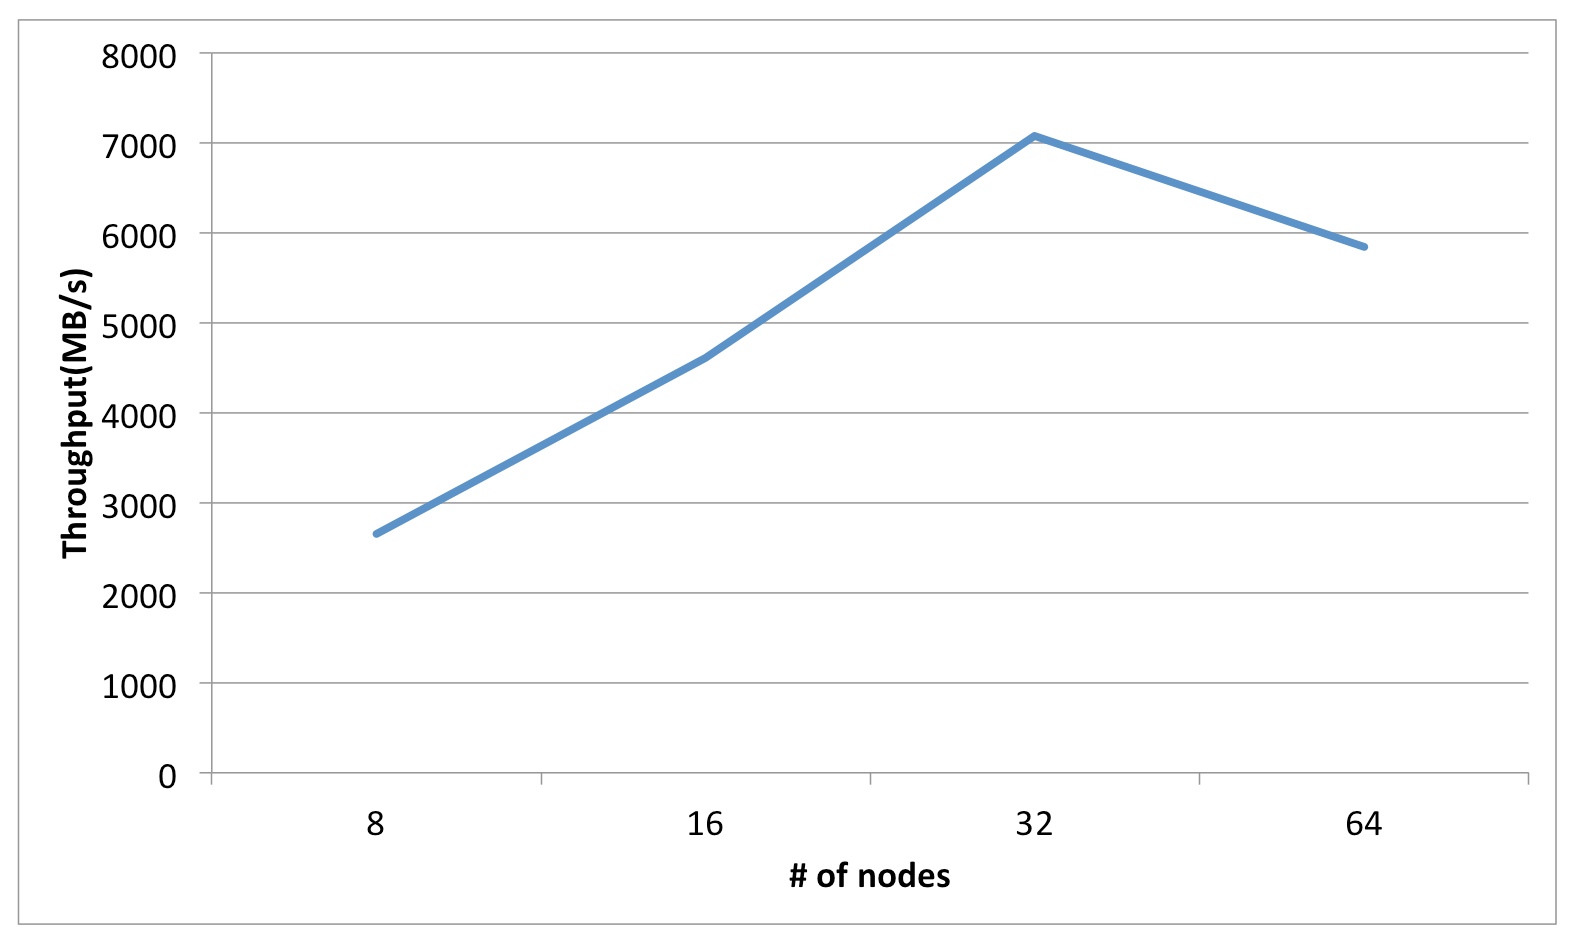
\includegraphics[width=6cm]{../img/throughput_tsubame}
	\caption{I/O Throughput to Lustre inside TSUBAME direct mount}
	\label{throughput TSUBAME}
\end{figure}

\begin{figure}[tb]
	\centering
	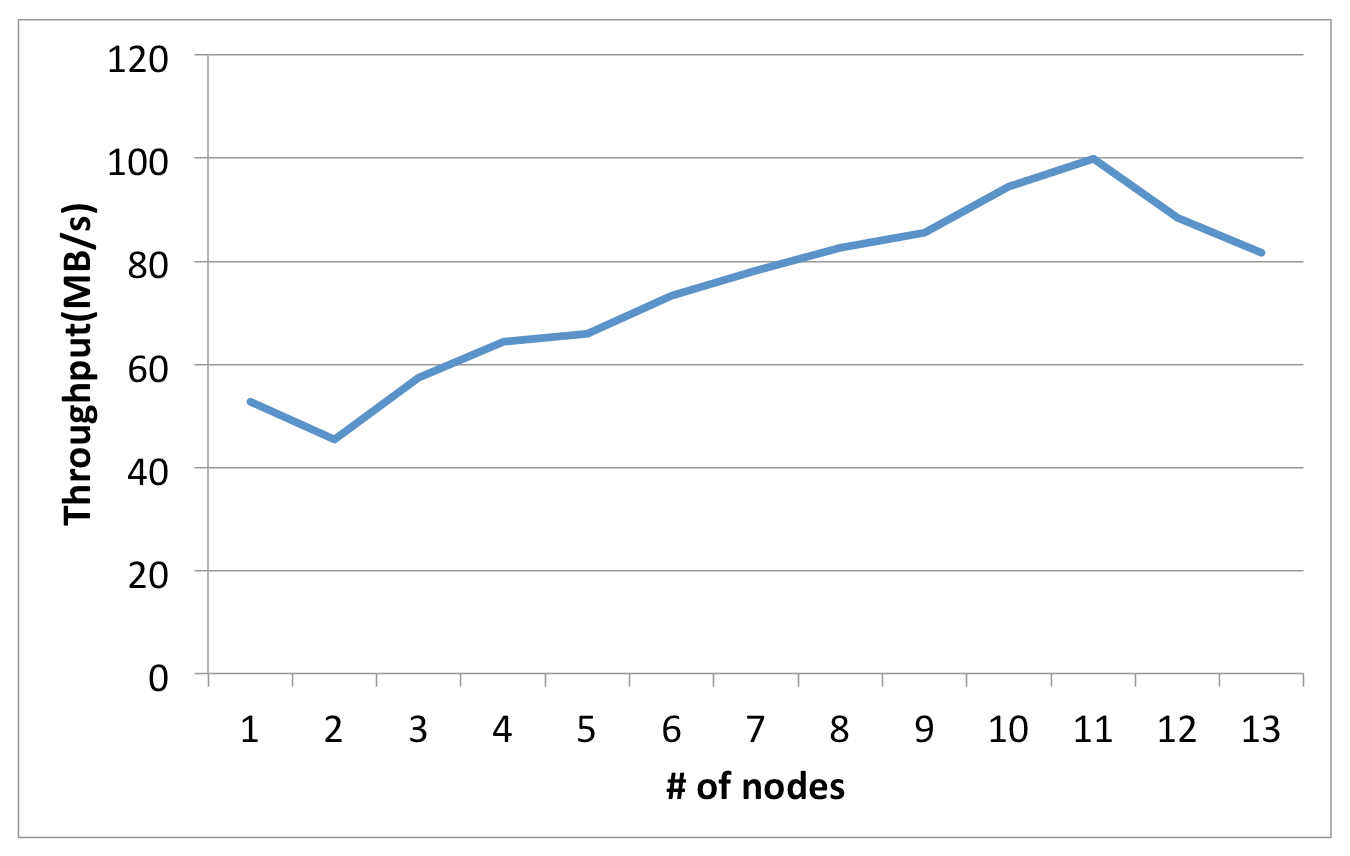
\includegraphics[width=6cm]{../img/AMAZON_to_OUR_LAB}
	\caption{I/O Throughput from AMAZON EC2 to file system inside our lab using sshfs}
	\label{throughput AMAZON to OURLAB}
\end{figure}

\begin{figure}[tb]
	\centering
	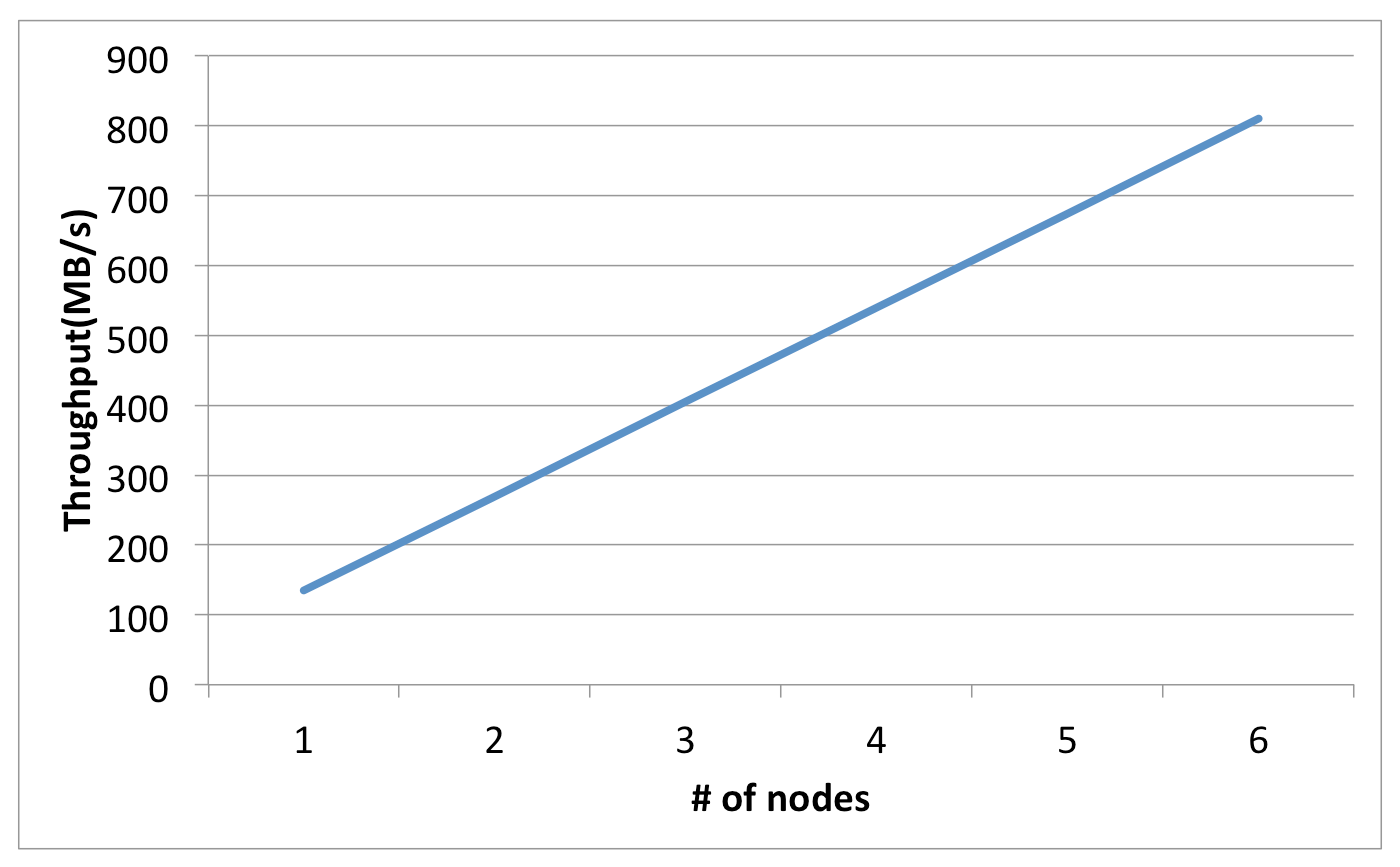
\includegraphics[width=6cm]{../img/point_to_point_AMAZON}
	\caption{point to point connection inside AMAZON}
	\label{point to point connection AMAZON}
\end{figure}

\begin{figure}[tb]
	\centering
	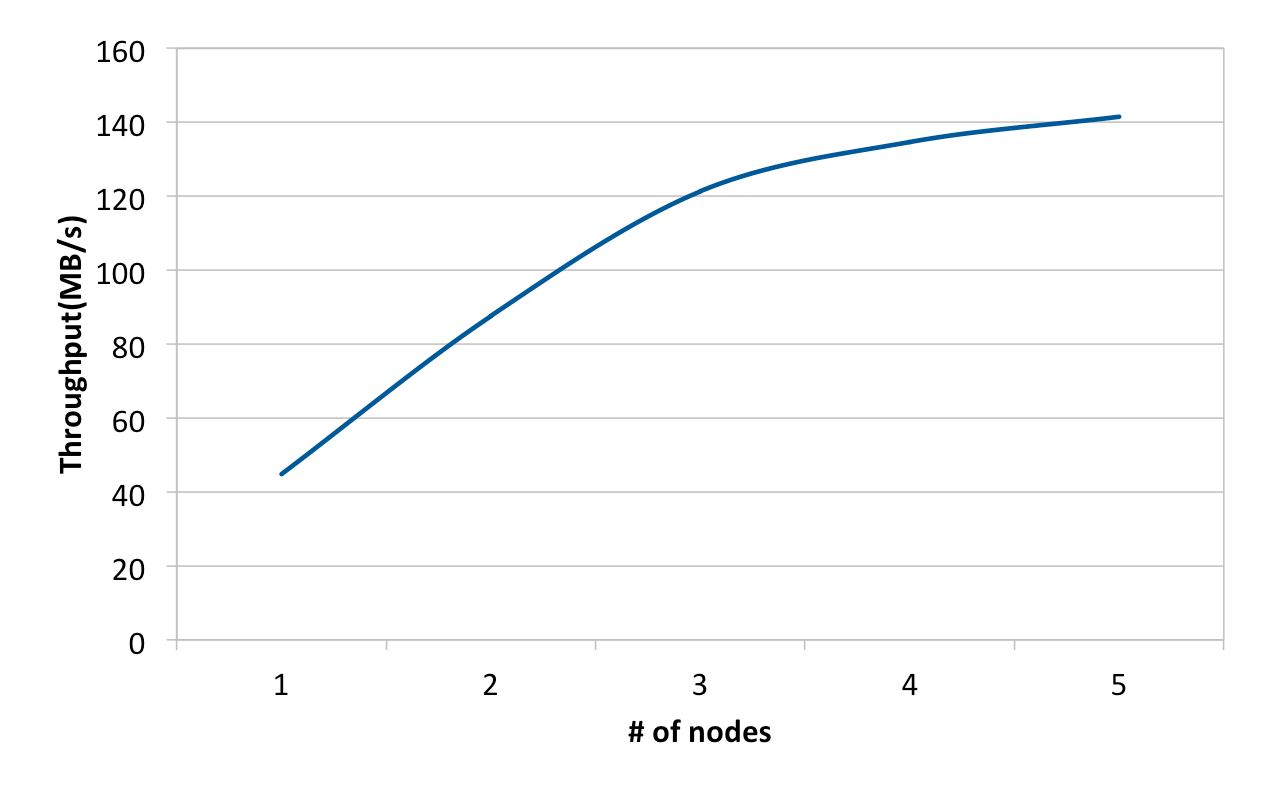
\includegraphics[width=6cm]{../img/point_to_point_lab}
	\caption{point to point connection throughput between AMAZON and our lab}
	\label{point to point connection LAB}
\end{figure}

\begin{table}[h]
\caption{\small TSUBAME thin node specification}
\label{tbl:spec}
\begin{center}
\begin{tabular}{|c|l|}
  \hline
  \cellcolor{lightgray} CPU      & Intel Xeon 2.93GHz CPU (4 cores)*2\\
  %(Hyperthreading enabled)\\
  \hline
  \cellcolor{lightgray} Memory   & 54GB (16 GB)    \\
  \hline
  \cellcolor{lightgray} SSD      & 120GB \\
  \hline
  \cellcolor{lightgray} GPU	 & NVIDIA Tesla K20X *3\\
  \hline
  \cellcolor{lightgray} Network  & QDR InfiniBnd *2 (80Gbps)\\
  \hline
\end{tabular}
\end{center}
\end{table}

\kento{Please explain what Public cloud is with example of Amazon EC2. Then, the details which is needed to mention for readers understand the rest of the sections.
  (1-1) Architecture (VM environment \& datacetners are geographically distributed)
  (1-2) Explain instance types which is related to this paper. Current draft does not mention any instance types.
  (1-3) introduce pay-as-you-go model to help readers understand the cost-based model in the modeling section 
  (1-4) [please add whatever you think it's needed]}
Public cloud is one in which the services and infrastructure such as applications and storage are provided off-site over the Internet, the main benefit of using a public cloud service are: easy fast and inexpensive set-up because hardware, application and bandwidth are covered by the provider, easy to scale to meet needs, no wasted resources because you pay for what you use.
There are many companies provide public cloud solution like google, IBM, Microsoft etc., among them, Amazon Elastic Compute Cloud (Amazon EC2)\cite{AMAZON_AWS} is one of the most famous public cloud, like other public cloud, Amazon EC2 privdes Virtualize computing, and owns computing and data centers in several geographic regions.
Amazon EC2 provide a large amount of instance types optimized to fit different use cases comprise varying combinations of CPU, memory, storage, and networking capacity.
In this study, we used general purpose m3.xlarge instance which has 4 vCPUs, 15GiB memory, 2*80GB SSD storage and high level Ethernet network condition in Tokyo region, we run Amazon Linux AMI 2014.03.2 (HVM), which is based on Linux 3.10 on these instances.
Amazon EC2 charges for nodes usage, Amazon use a pay-as-you-go pricing policy\cite{AMAZON_AWS}, which means you pay only for what you use, there is no minimum fee and you will pay for compute capacity by the hour with no long-term commitments.
\subsection{Federation between supercomputers and clouds}
\kento{Please explain (2-1) how we federate supercomputers with clouds. $=>$ Virtualize supercomputer (e.g. TSUBAME V) + VM on clouds. 
                      (2-2) what the advantages are. $=>$ VMs can provide the same execution environment on both supercomputers and clouds
                      (2-3) [please add whatever you think it's needed]}
When we try to federate supercomputer with public clouds, there are need to have a similiar performance and environment between these two systems.
So we virtualize the supercomputer(like TSUBAME V queue) and federate VMs running on supercomputers with VMs provided by public cloud.
By using VMs, we can run the same image on both supercomputer and public cloud as well as set both the same specification, and make it looks the same to user.%we can use in order to get the same execution environment on both supercomputers and clouds, we virtualize supercomputer, e.g. TSUBAME V queue with VM on clouds.
\subsection{Challenges in Federation with clouds}
\label{sec:problems}
\kento{In this section, (3-1) First explain I/O problems in federation with clouds based on the cloud architecture explained in the above (1-1) as well as using Fig.1-4. 
                        (3-2) Then, please briefly clarfy why ``(A) I/O burst buffer`` can improve I/O performance without using model. For example, parallel I/O, cacheing .... 
                              (Remember we knew that I/O burst buffer is effective before compareing the performances between w/ and w/o burst buffers by using performance model)
                        (3-3) Another challenge is a choice of instance types for burst buffer, and understanding the trade-off between I/O perfomrance and the monetary cost. 
                              In addtion, the choice of instances, the trade-offs are changes depending on given a supercomputer and cloud environments, such as network throughput, PFS performance. 
                              That's why the ``(B) perfomrance modeling`` is important}
Although we virtualize supercomputer and obtain a similiar environment on both supercomputers and clouds, there are still several problems remains, for example, input data of applications running on supercomputer is usually stored in shared storages in the same system and can be read from and wrote to these storages with a extremely high throughput.

We use Iperf\cite{iperf}, which was developed by NLANR/DAST as a modern alternative for measuring TCP and UDP bandwidth performance, and IOR\cite{IOR}, which is widely used for benchmarking parallel file systems using POSIX, MPIIO, or HDF5 interfaces.
Fig.~\ref{throughput TSUBAME} shows read and write throughput from TSUBAME V queue nodes (VM runing on TSUBAME Thin node, which specification is shown in \tabref{tbl:spec}) and TSBUAME Lustre file system, which is mounted by using lustre client, it is a interconnection throughput inside TSUBAME supercomputer, we can see that I/O throughput growing as numbers of nodes growing, and the aggregate read and write throughput reach 6-8GB/s with 64 nodes, the same result also can be seen in \cite{checkpointing}.
However, Fig.~\ref{throughput AMAZON to OURLAB} shows I/O throughput between AMAZON EC2 nodes and a file system machine inside our lab, since TSUBAME Lustre can not be accessed outside of TSUBAME because of security problem, instead of TSUBAME Lustre file system, we used a file server inside our lab, which has 1GBit/s internet bandwidth, also because of security problem, we used sshfs\cite{sshfs},which is a filesystem client based on SSH File Transfer Protocol, to mount this file system from Amazon.
We can see that the I/O throughput also grows as number of nodes grows but the aggregate throughput is only 100-140 MB/s, which is limited by Internet bandwidth, about 40-80 times smaller than throughput inside TSUBAME.
For data-sensitive application, low I/O throughput is devastating, especially for application running on supercomputers, furthermore, lower I/O throughput leads a longer execution time, according to Amazon pay-as-you-go policy, longer execution time means more cost.

However, when we look at Ethernet throughput inside Amazon as Fig.\ref{point to point connection AMAZON} shows, although we only show the result up to 8 pairs of nodes, each node achieved only 135MB/s (1GBit/s), the influence between nodes is extremely small, figure shows a perfect linear line also a strong scalability.
since when we running the benchmark, many other users were also running applications on Amazon, so we can assume that highest throughput 1GB/s (8Gbit/s) shown in Fig.~\ref{point to point connection AMAZON} is not the maximum bandwidth of Ethernet in Amazon EC2 .
Comparing Fig.~\ref{point to point connection AMAZON} with Fig.~\ref{throughput AMAZON to OURLAB} and Fig.~\ref{point to point connection LAB}, Ethernet throughput is much higher than Internet, it shows that our solution, by using I/O buffer nodes can achieve a higher Ethernet throughput than Internet.

To solve this problem, we propose our I/O burst buffer architecture, since usually Internet throuhput is the bottleneck, by using parallel I/O and cacheing file in I/O buffer nodes, we can fully utilize the Internet bandwidth as well as avoid frequently transfering file between two systems, hence achieve a high I/O throughput.
Althought using I/O buffer can increase I/O throughput, reduce the execution time and cost, I/O buffer nodes will be charged for usage, also a better instance will cost more than a normal one, there will be a trade-off between I/O performance and monetary cost, we will introduce a throughput-based model and a cost-based model to predict the throughput and overall cost.
%Moreover, the instance choice, number of I/O nodes depends on supercomputer and pulic cloud environment, in our following section, we will provide a performance modele

%when we try to move some jobs to public clouds after federation, the data 
\kento{Then, in the rest of the section, we explain (A) and (B)}


%\subsection{(Current Section 2)}
\kento{Please fit the below sentences to the above sections with additional explanations}

% vector figures
% Fig. 4 does not have a frame
% write machine spec 

%When people analyze large size of data, parallel programme is widely used in order to reduce computation time, especially when using supercomputer.
%However, it is usually difficult for a non-computer-scientist to write a parallel program, or re-write some existing applications into parallel version.
%Many serial applications are submitted to Supercomputer and occupy computing nodes for a long time, causing other applications which offer large number of nodes to wait for nodes, and leading a low utilization of computing resource.
%Consider following situation, there are 50 nodes available when a user submits a serial program using 1 node for 4 hours, after an hour a user try to run a program using 50 nodes, then he can't start his program until the first user finished his job.
%Such situation happens frequently when thousands and hundreds of users using one system at the same time and leading a low utilization of computing resource.
%One solution is running several virtual machines on a single physical machine for increasing utilization, which is used in TSUBAME Supercomputer, but sometime it still can't meet the request.
%For request not always reaches peak, it is not wise to increase nodes just for a temporary request peak.
%However even using virtual machines computing nodes still can't meet the request of users, for example, power problem will be critical in summer and nearly half of computing nodes have be shut down to reduce electricity consumption in the case of TSUBAME Supercomputer.
%Facing these problems, one solution will be federate supercomputer with public cloud.
%By using public cloud computing nodes just in request peak or when facing with power problem, people can save cost for buying new machines.
%Of cause, there will be many challenges when Supercomputer federates with public cloud, such as security problems, using public cloud may cause research data opened to public, also connecting with Internet put Supercomputer under threats of hacker's attack.

%Data shown in this section is taken from AMAZON EC2 m3.medium nodes, which have 3.75GiB memory and Moderate Network Performance and TSUBAME 2.5 V queue, which uses VM.


%Fig.~\ref{throughput TSUBAME} shows I/O throughput between TSUBAME V queue nodes \kento{Describe node specification in Table I}(VM runing on TSUBAME Thin node, which specification is shown in \tabref{tbl:spec}), which run on VM on several shared machines and TSBUAME Lustre file system, which is mounted by using lustre client, it is a interconnection throughput inside TSUBAME supercomputer, we can see that I/O throughput growing as numbers of nodes growing, and the aggregate read and write throughput reach 6-8GB/s with 64 nodes, the same result also can be seen in \cite{checkpointing}.
%On the other hand, Fig.~\ref{throughput AMAZON to OURLAB} shows I/O throughput between AMAZON EC2 nodes and a file system machine inside our lab, which has about 1GBit/s Internet access.
%From Fig.~\ref{throughput TSUBAME} and Fig.~\ref{throughput AMAZON to TSUBAME Lustre} we can see that the I/O throughput of interconnection inside supercomputer is quit larger than that from AMAZON.
%Also, if we compare the one nodes I/O throughput, 
%Also if we compare Fig.~\ref{point to point connection LAB} with Fig.~\ref{throughput AMAZON to OURLAB}, the maximum throughput \kento{??}
%If we move some jobs to AMAZON EC2 with input data stored in TSUBAME Lustre, the execution time will increase because of I/O low throughput,for a data sensitive application, it will be devastating, also according to AMAZON's pay-as-you-go policy\cite{AMAZON_AWS}, longer execution time means more cost.

%But when we compare Fig.~\ref{point to point connection TSUBAME} with FIg.~\ref{point to point connection AMAZON}, the interconnection throughput 

%using I/O burst buffer requires addtional nodes running on public cloud and means more cost, also like Amazon EC2, public cloud usually provides various instance types with different specification, using which instance type also will affect both cost and performance.
%We provide a cost-based model to determine 
%Since we can achieve a high interconnection throughput inside a system (HPC system, public cloud), we consider use some nodes as a buffer nodes, using a buffer queue to buffer I/O data and achieve a high throughput.

%Although there are some studies about workflow optimization and  balance\cite{Workload}, Since data transfer rate is extremely low in Internet compared with interconnection network and data size processed is extremely large, user do not want to settle their nodes across two systems, so in this model, we just consider the situation that all nodes used for the same job are allocated in the same system.


%3
\section{I/O Bursting Buffer Overview}
\label{sec:burst_buffer}

%\begin

An overview of I/O burst buffer architecture and two kinds of connection: direct connection and I/O bursting buffer are described in this section.
As we mentioned in the previous section, our model takes advantage of high throughput inside a system, and use buffer queue system in order to increase throughput between two systems.
The main idea is that some of computing nodes serve as a I/O buffer nodes in each system, I/O data will first be buffered in buffer queue in the same system, and then be transferred to final storage system.
%the same computing nodes and then these I/O buffer nodes, after that data will be  transferred to storage in another system.
Two kinds of buffer are used in our I/O burst buffer architecture, the first one is in client computing node, first buffer user I/O in the same node, another one is in I/O buffer nodes.
%Although our goal here is to federate supercomputer with public cloud, since there are a great performance gap between normal supercomputer nodes and public cloud nodes and problem described above, here we consider about federating virtual machine nodes which running on supercomputer physical nodes with public cloud.
%Since public clouds also run virtual machine on physical nodes, in the follow section, we treat the set of supercomputer's virtual machines as a cloud environment, also because only a few public IP address available in each cloud, I/O buffer nodes are required even in direct connection model.


%Reading operation describes operations when issues reading data from another cloud storage, and writing operation describes operation when issues writing data to another cloud storage

%Migration operation occurs when some nodes have to be shut down in one cloud 
%all jobs running on these nodes have to be backed up by using snapshot, 

\subsection{System Environment}
First a general system used in following sections is defined as follow:

%For security consideration and the fact that IPv4 addresses becomes rare,
\begin{itemize}
	\item All computing nodes are connected by large bandwidth and interconnection network, note network topology maybe different in each system, so topology is not specified here, interconnection network performance is measured by throughput.
	\item There are a constant number of public IP addresses can be assigned to some computing nodes.
	\item There is a shared storage for date sharing inside system, all computing nodes are connected with shared storage, also the filesystem of shared storage is not specified and performance is measured by throughput.
\end{itemize}

\subsection{I/O Burst Buffer Architecture}

\begin{figure}[tb]
	\centering
	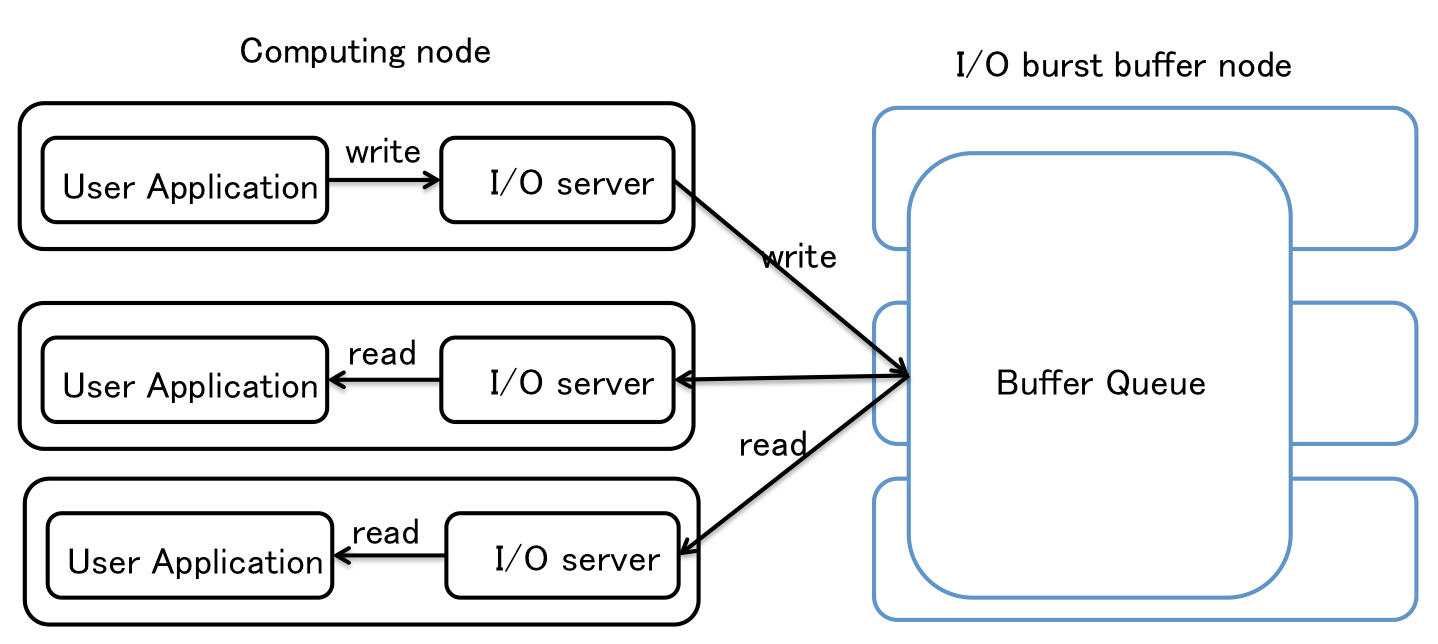
\includegraphics[width=6cm]{../img/IOserver}
	\caption{I/O server and buffer queue}
	\label{I/O server}
\end{figure}

\begin{figure}[tb]
	\centering
	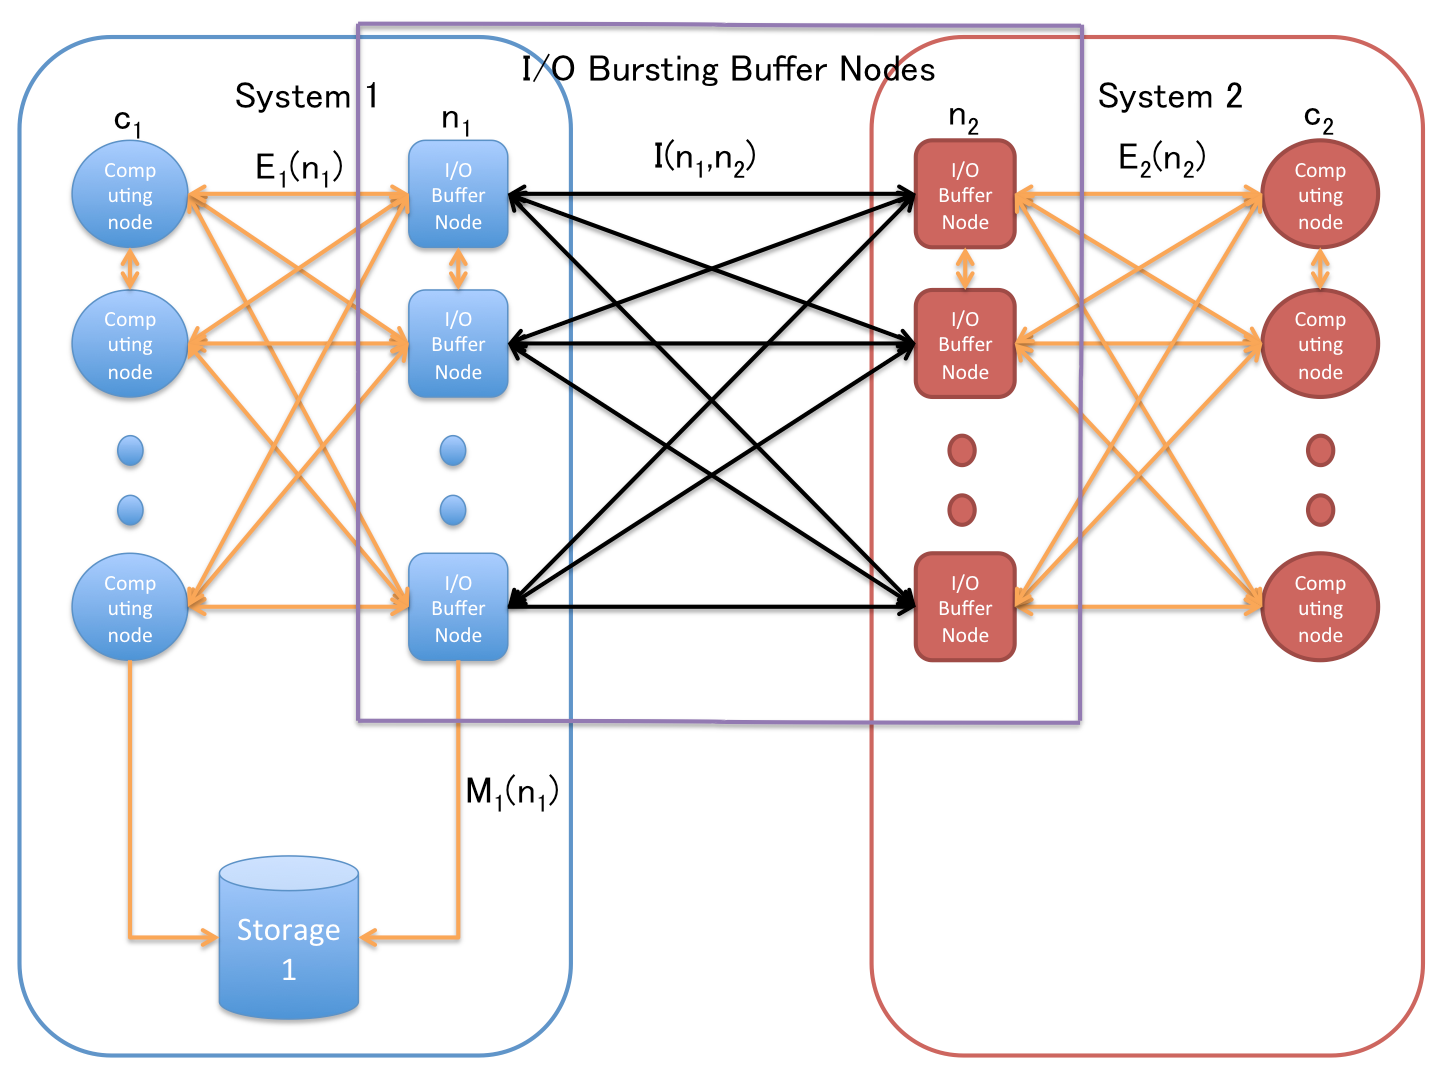
\includegraphics[width=6cm]{../img/overview}
	\caption{overall illustrate of I/O Burst Buffer Architecture}
	\label{overview}
\end{figure}

%Fig.~\ref{overview} and Fig.~\ref{I/O server} are the overall illustrate of I/O Bursting Buffer:
There are two kinds of nodes in our I/O burst buffer architecture: \emph{computing nodes} and \emph{I/O burst buffer nodes}, computing nodes run user's application,which assigned only  and I/O burst buffer nodes, which assigned both private IP address.

Fig.~\ref{I/O server} is a illustrate of I/O server inside client nodes and buffer queue in I/O burst buffer nodes.
In each computing node, there is a I/O server, which is a filesystem client used to buffer I/O data and send to or read from I/O buffer nodes.
Among I/O burst buffer nodes, there is a master nodes, which maintain a global buffer queue and a namespace, controll buffer read and write, and manage I/O buffer nodes, buffer data is distributed to all I/O buffer nodes in order to enable concurrent read and write.

When a user application issue a write request, I/O data will be buffered in that node by I/O server, when user close the file, call flush function or I/O data size exceed I/O server buffer size, I/O data will be transferred to I/O burst buffer.
First, I/O server sends the size of I/O data to master I/O burst buffer node, master node return a list of several I/O buffer nodes, then I/O server split I/O data into pieces, and sends each pieces to a I/O buffer node, after data transfer finished, that file will be added to buffer queue and namespace, and this file can be seen by all computing nodes, since we assume that all nodes used by the same job are allocated in the same system, so data consistency can be guaranteed since that.
Buffer queue operation including data write back and operation when queue is full will be described in following section.

When user issue a read request, there are two conditions: file is buffered in buffer queue in I/O burst buffer, or file is stored only in storage in another system.
In the first cases, file can be transferred to computing nodes from buffer queue directly, and can achieve a high throughput.
If data is not in buffer queue, then a read operation described below will be executed, since data must be transferred from storage in another system, in this case, throughput will depend on Internet condition and it is hard to achieve a high throughput.

Fig.~\ref{overview} shows a overall illustrate of I/O burst buffer architecture.

%Consider there are two systems, named system 1 and system 2


%Arrows stand for network connection.
%Orange arrows are interconnection networks inside cloud, although two clouds used the same color for interconnection networks, bandwidth can be different, also the topolopies are not specified and can be different in each cloud.
%Black arrows are Internet connections, since there are a few amount of public IP addresses available, only I/O buffer nodes are connect to Internet, also the amount of available public IP address becomes the upper bound of the amount of I/O buffer nodes in each cloud. 
%Although nodes with private IP address can use route or other net device to connect to Internet, but consider about security problem, also using route will reduce concurrent data transfer rate, here we assume all nodes in cloud only connect to local private network except I/O buffer nodes which connect to both local network and Internet.

%Circles stand for computing nodes, which are used for standard computation.
%Here we assume all computing nodes can communicate with each other, and also I/O buffer nodes and shared storage in the same cloud environment.
%Squares are I/O buffer nodes, these nodes are used for data transfer between clouds, and are assigned with both public and private IP addresses.
%I/O buffer nodes can use the same machine or VM as computing nodes, or can use network optimized nodes for larger throughput, but it is not required here.
%Cylinders are shared storages, which are used to store data used by computing nodes, usually shared storage is consist of several nodes with a distributed filesystem and uses a better network, offers a large throughput.

%Since there is a big gap between cloud inside data transferring and accross two clouds in throughput, our goal is to fill the gap. 

%For convenience, in the following section we assume data is stored in Cloud 1's shared storage, and computing nodes in Cloud 2 are used for computation. 

%in this subsection, we introduce operations of buffer queue write back.

\subsection{Read and Write}

\begin{figure}[tb]
	\centering
	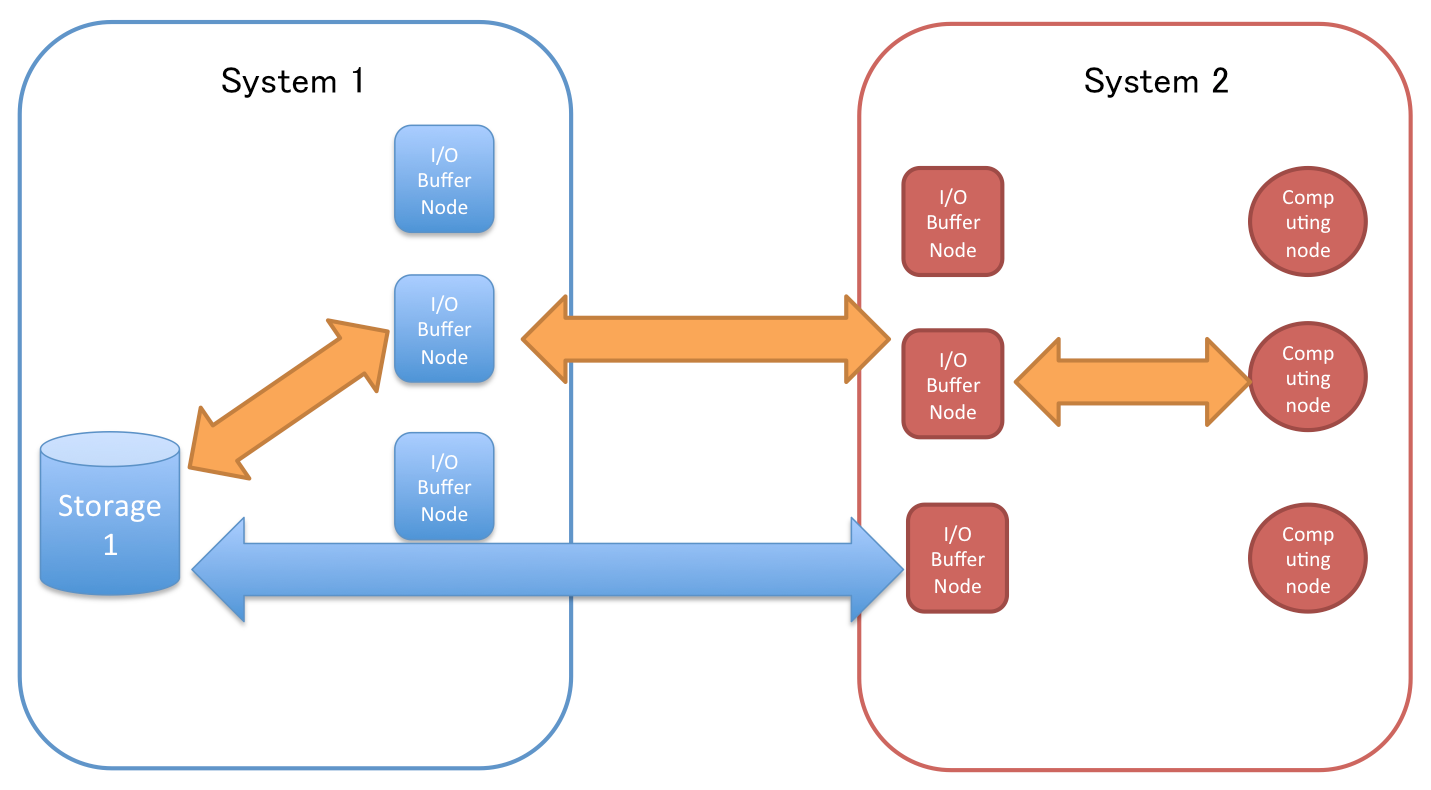
\includegraphics[width=6cm]{../img/read_and_write}
	\caption{read and write operation}
	\label{read and write}
\end{figure}

In this section we describe operations when file is not in I/O buffer nodes or file needs to be write back to storage in another system.
We propose two kinds of model: one-side buffer and two-side buffer.

\subsubsection{One-side Buffer}

As Fig.~\ref{read and write} blue arrow shows, one-side buffer is a connection between I/O buffer nodes in system 2 and storage in system 1 directly.
When I/O nodes need to write data back to storage in another system, since data is already spread among I/O nodes, a parallel write can be achieve to fully utilize the Internet bandwidth.

Similarly, when I/O nodes need to read data from storage in another system, several I/O nodes will be assigned equal size of data, and then these nodes read assigned piece of data from the storage concurrently.

There will be two problems in this solution:
\begin{itemize}
	\item First storage should be opened to Internet, in order that I/O nodes can read from or write to it.
		However storage system in supercomputer store Petabyte of research data, open the access of storage system means that put these research data under risk of attack.
	\item As we mentioned before, throughput of one side communication is lower than two side communication, since we use SSH protocol based File system for security reason.
		also two side communication can achieve a higher throughput with fewer nodes, according to pay-as-you-go policy, reduce number of nodes can reduce cost.
\end{itemize}
%data firstly be splitted into number of I/O buffer nodes in cloud 2 pieces and assign one I/O buffer node one piece, then I/O buffer nodes start reading assigned data concurrently in order to fully utilize Internet bandwidth.
%After reading finished, I/O buffer nodes send data to each computing node Simultaneously, there data will be restructure by using protocol described below.

%Like reading, when computing nodes start to output data, first data will be buffered inside that nodes.
%After output finished, data will be splitted into number of I/O buffer nodes in cloud 2 pieces, and assign one I/O node one piece, then data will be sent to all I/O buffer nodes concurrently.
%When I/O buffer nodes received data, then they writing data back to storage in cloud 1.

\subsubsection{Two-side Buffer}

On the contrary, two-side buffer solution use I/O buffer nodes in both two systems as Fig.~\ref{read and write} orange arrows show.
I/O data will be split twice, transferred throughput two sides of I/O buffer nodes and then reached the destination.

Consider I/O nodes in system 2 issue a write back operation, also, data is already spread among I/O nodes in system 2, each I/O node will find a pair among I/O nodes in system 1, then transfer their piece of data to system 1 concurrently.
After I/O node in system 1 received data, they write data back to storage in system 1.

Compared with one-side buffer, two-side buffer required one more data transfer (I/O nodes to storage in the same system), if storage data transfer throuhput become a bottleneck, two-side buffer will cost more time than one-side buffer.
Also, two-side buffer require both systems allocate I/O buffer nodes, if node usage is charge in both system, total cost may be larger than one-side buffer.

%the bottleneck is still Internet throughput, since interconnection is far faster than Internet.
Since two-side buffer does not read data from or write data to storage directly, it means we can compress data before transfer it, though it will take some time to compress and decompress data, when the Internet throughput is extremely low, compress and decompress time will be far smaller than tranferring time, and compress data can make more data buffered in buffer queue.
Also, unlike one-side buffer, two-side buffer do not require storage to be opened to Internet, only required several I/O nodes have access to Internet.

%I/O bursting buffer model may be used when throughput of direct connection between I/O buffer nodes and storage in different cloud is smaller then throughput between I/O buffer nodes, it is possible when storage is consist of few nodes, and direct connection will be 1-N connection, on the contrary, connection between I/O buffer nodes is N-N connection, has larger parallelism.

%When computing nodes issue read request, first we check whether the file has been cached in I/O buffer nodes in cloud 1, if not, File will be splitted into the same number of I/O buffer nodes in cloud 1, and each I/O buffer node will be assigned a piece of split, then all I/O buffer nodes start reading assigned piece of data from shared storage simultaneously to fully utilize the bandwidth.% I/O buffer nodes use a main index to refer to the data position in global data.

%After transferring data from shared storage finished, I/O buffer nodes in cloud 1 will connect with all I/O buffer nodes in cloud 2, then split data piece and into number of I/O buffer nodes in cloud 2,
%here a sub-index is used to refer to each piece's position, 
%then transfer these pieces to I/O buffer nodes in cloud 2 concurrently in order to fully utilize Internet bandwidth.

%When data transfer finished, I/O buffer nodes connect with all computation nodes which needs data, then transfer data to the corresponding position by using a index protocol described below, of cause all data transfer are done in parallel.

%Data writing operation doing the opposite operation as reading operation.
%When a computing node in cloud 2 issues data writing, output data will be first buffered by I/O server in that node.
%After output finished, I/O server connects with all I/O buffer nodes in the same cloud, and split output data into the number of I/O buffer nodes, then send each piece of data to each I/O buffer nodes Simultaneously.

%I/O buffer nodes then again split data into the number of I/O buffer nodes in cloud 1, like reading operation, here sub-index is used to refer to data position. and then start to transfer data concurrently. 

%Then I/O buffer nodes write data to storage in cloud 1.



\begin{comment}
\subsubsection{Index Protocol}

\begin{figure}[tb]
	\centering
%	\includegraphics
	\caption{index protocol}
	\label{index protocol}
\end{figure}

As Fig.~\ref{index protocol} shows, two indexs are used in this protocol: main index and sub-index.
There are two phases of data splitting in both reading and writing operation, 
\end{comment}
%\subsubsection{Node Migration}
%Node migration happens when some nodes have to be shut down due to some situation like power problem in summer, and still need to provide service to users.
%In these cases, nodes will be migrate by snapshot, usually snapshots of these nodes will first be stored into shared storage, then these snapshots will be transferred to another cloud, and start VM by using these snapshots.

%However, the low throughput between direct connection of nodes and storage in different environment will still be a bottleneck for quick migration.
%When using I/O buffer nodes 


\section{I/O Burst Buffer Model}
\label{sec:model}
\kento{First, again mention why the modeling is important for reminder}
%\begin{figure}[tb]
%	\centering
%	\includegraphics
%	\caption{definition}
%	\label{definition}
%\end{figure}

The throughput-based model, cost-based model and buffer queue write back model are described in this section.
As we explained in the previous section, two-side buffer model is better than one-side buffer model, in the following section, we will use two-side buffer model as our read from and write back model in I/O burst buffer
\kento{this sentences should be in the previsou section}.

The throughput-based model compares throughput with and without I/O burst buffer, cost-based model compare cost with and without I/O burst buffer, and buffer queue write back model shows the situation that I/O buffer queue will be full. 
We make definitions shows in Table \ref{definition} in order to describe our model.
\begin{table}[tb]
	\caption{Definition of parameters}
	\label{definition}
\begin{tabular}{|p{3cm}|p{5cm}|}
	\hline
	$c_1,c_2$&Numbers of computing nodes in system 1 and system 2\\\hline
	$n_1, n_2$&Numbers of I/O buffer nodes in system 1 and system 2.\\\hline
	$m_1,m_2$&Available memory size for each I/O node in system 1 and 2, also the maximum buffer size will be $n_1\times m_1$ and $n_2\times m_2$\\\hline
	$D_1(n_2),D_2(n_2)$&Throughput when $n_2$($n_1$) I/O nodes in system 1 (system 2) connect to storage in the other system directly, here we assume I/O nodes and computing nodes in each system have the same Internet connection speed.\\\hline% have Internet connection.\\\hline
	$I(n_1,n_2)$& 	Internet throughput using $n_1,n_2$ nodes respectively, since overall Internet throughput is affected by number of nodes involved in connection.\\\hline
	$E_1(n_1), E_2(n_2)$&Interconnection network throughput in system 1 and 2, although interconnection throughput is also affected by numbers of I/O nodes and computing nodes, numbers of users will running application on different number of computing nodes.\\\hline
	%, it is difficult to compute each throughput, so here we use $E_1(n_1)$ to refer to limitation of maximum throughput of interconnection network in system 1 with $n_1$ I/O nodes, likely ,$E_2(n_2)$ is limitation of maximum throughput of interconnection network in system 2 with $n_2$ I/O nodes.
	$M_1(n_1),M_2(n_2)$& Throughput of connection between storage and $n_1$ I/O nodes in system 1 and storage and $n_2$ I/O nodes in system 2.\\\hline
	$C_i\_Money(T)$& Cost for standard node in system $i$ for $T$ time usage\\\hline
	%and cost for node in system 1 is $C_2\_Money(T)$ for $T$ time usage, and since I/O nodes may use a better network, 
	$C_i\_High\_Money(T)$ &I/O nodes in system $i$ for $T$ time usage, since I/O nodes may use a better network condition, we assume it will cost more than normal nodes.\\\hline
\end{tabular}
\end{table}

\subsection{Throughput-based Model}
%There are many facts will affect throughput of Internet, so here a moniter is used to evaluate throughput between 
In the case of direct I/O \kento{What is direct I/O. I think it means direct connection mode in Section 3, but no explanation at all}, computing nodes connect to storage in another system directly, there is only one data transfer, so throughput \kento{read ? or write ? or both ?} will be:%there are two data transfers: computation nodes to I/O buffer nodes in system 2, I/O buffer nodes in system 2 to storage in system 1, so throughput will be:
\begin{equation}
	\text{thr}_{\text{direct}}=D_1(c_2) \label{throughput1}
\end{equation}

When using I/O burst buffer, there will be three data transfers: computation nodes to I/O buffer nodes in system 2, I/O buffer nodes in system 2 to I/O buffer nodes in system 1, I/O buffer nodes in system 1 to storage in system 1, throughput \kento{write ? and read ?. Explain how the buffer queue works (1) if buffer space is avaialble for write, (2) reading data is in the buffer queue. We need expian this in both previous section and in here} will be:
\begin{eqnarray}
	\text{thr}_{\text{I/O buffer}}=\begin{cases}
		E_2(n_2) &\text{buffer queue available}\\ 
	\min\{M_1(n_1),I(n_1,n_2),E_2(n_2)\} &\text{buffer queue full}
	\end{cases} \label{throughput2}
\end{eqnarray}

In this throughput-based model, these two throughputs are evaluated, and a switch is based on these two values:
\kento{Why do you swithches between direct I/O and burst buffer?}
\begin{equation}
	\begin{cases}
		\text{thr}_{\text{direct}} \geq \text{thr}_{\text{I/O buffer}} & \text{use direct I/O}\\
		\text{thr}_{\text{direct}} < \text{thr}_{\text{I/O buffer}} & \text{use I/O burst buffer}
	\end{cases}
\end{equation}

\kento{Mention how do you switch between I/O burst buffers and direct I/O. Will you dynamically shutdown/boot burst buffer nodes on demain ?. If so, please explain so, but there is a time lag before shutdown/boot are completed. So say somthing like "We will solve the problem in future work'' or else}

\subsection{Cost-based Model}
\kento{Again, it's hard to understand due to lack of information. Please read carfully over and over again and add more explanation like in the above}
In the case of cost-based model, we consider the overall cost for using direct I/O and using I/O burst buffer. Although using I/O burst buffer will cost for I/O nodes, higher throughput can reduce execution time and also overall cost.
using \ref{throughput1},and \ref{throughput2} total time for transferring unit size of data can be compute as:

\begin{equation}
	\begin{cases}
		T_1=\frac{1}{D_1(c_2)} & \text{direct}\\
		T_2=\frac{1}{\min\{M_1(n_1),I(n_1,n_2),E_2(n_2)\}} &\text{buffer queue available}\\
		T_3=\frac{1}{E_2(n_2)} &\text{buffer queue full}
	\end{cases}
\end{equation}

here we compute cost by using $T_1,T_2,T_3$:
\begin{equation}
	\text{cost}_\text{direct}=c_2\times C_2\_Money(T_1)+n_2\times C_2\_High\_Money(T_1)
\end{equation}
\kento{According to the difinition of $C_i\_Money(T)$ and $T_i$, the above model seems to be wrong. Please read carfully the model is correct}
\begin{align}
	\text{cost}_\text{I/O buffer}=\\\begin{cases}
				c_2\times C_2\_Money(T_2)+n_1\times C_1\_High\_Money(T_2)+n_2\times C_2\_High\_Money(T_2)&\text{buffer queue available}\\
				c_2\times C_2\_Money(T_3)+n_1\times C_1\_High\_Money(T_3)+n_2\times C_2\_High\_Money(T_3) &\text{buffer queue full}
\end{cases}
\end{align}

In this cost-based model, these two cost are evaluated, and a switch is based on these two values:
\begin{equation}
	\begin{cases}
		\text{cost}_{\text{direct}} \geq \text{cost}_{\text{I/O buffer}} & \text{use direct I/O}\\
		\text{cost}_{\text{direct}} < \text{cost}_{\text{I/O buffer}} & \text{use I/O burst buffer}
	\end{cases}
\end{equation}

\kento{I'm workding if the throuput is 	$\text{thr}_{\text{direct}} < \text{thr}_{\text{I/O buffer}}$ the cost is $\text{cost}_{\text{direct}} \geq \text{cost}_{\text{I/O buffer}}$, which do you use, direct I/O and I/O buffer.}

%\subsection{}
%\subsection{Migration Model}
%Since there are some condition that some supercomputer nodes must be shut down, and jobs running on these nodes have to be migrate to another cloud. There are 
%\begin{equation}
%	Data	
%\end{equation}
\subsection{Buffer Queue Write Back Model}

\begin{figure}[tb]
	\centering
	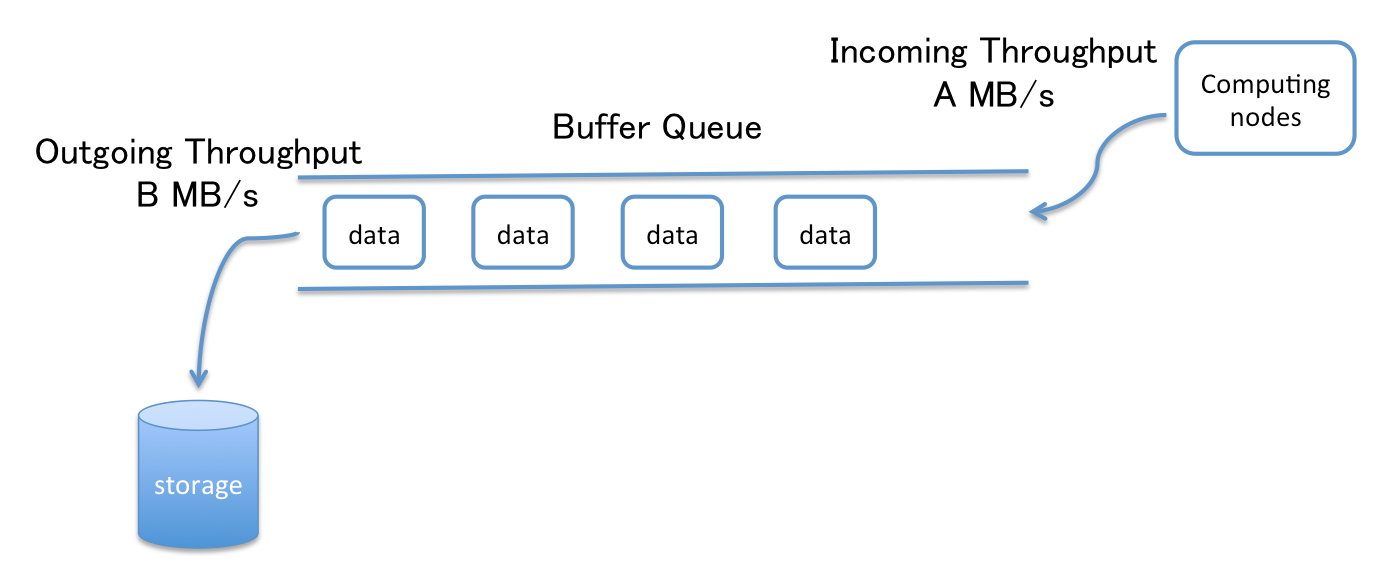
\includegraphics[width=6cm]{../img/buffer_queue}
	\caption{buffer queue}
	\label{buffer queue}
\end{figure}

If the buffer size is unlimited. then we can buffer all data in the I/O buffer nodes, and achieve a high throughput in cloud burst \kento{Good work !! As I said in the different sections, it's important to remind its motivation before describing the algorithm, techniques, model, or methods for its reminder}.
However buffer size can not be unlimited, we can not buffer all data in the I/O buffer nodes, data in buffer nodes have to be write back to storage in another system.
The problem is which data should be written back to storage, like cache in cpu, if we can reduce cache miss in this situation, we can increase throughput. 
According to data locality, we use a priority queue to determine which data should be write back.

Consider Fig.~\ref{buffer queue}, assume average incoming throughput is A MB/s and average outgoing throughput is B MB/s, if A always larger than B, after $T$ time buffer queue will full.
\[T=\frac{m_2\times n_2}{A-B}\]

After that, since buffer queue is full, I/O server can not send more data to I/O buffer nodes, have to block any read and write request since that.
In this case, jobs running on public cloud have to be moved back to original system until buffer queue is empty
\kento{Why ??}.


\section{Evaluation}
\label{sec:evaluation}

\begin{figure}[tb]
	\centering
	\includegraphics[width=6cm]{../img/throughput_comparison}
	\caption{throughput comparison with and without I/O burst buffer}
	\label{throughput comparison}
\end{figure}

\begin{figure}[tb]
	\centering
	\includegraphics[width=6cm]{../img/cache_hit_rate_throughput}
	\caption{throughput comparison between each cache hit rate}
	\label{throughput cache rate}
\end{figure}

\begin{figure}[tb]
	\centering
	\includegraphics[width=6cm]{../img/maximum_throughput}
	\caption{maximum avaliable throughput}
	\label{maximum throughput}
\end{figure}

\begin{figure}[tb]
	\centering
	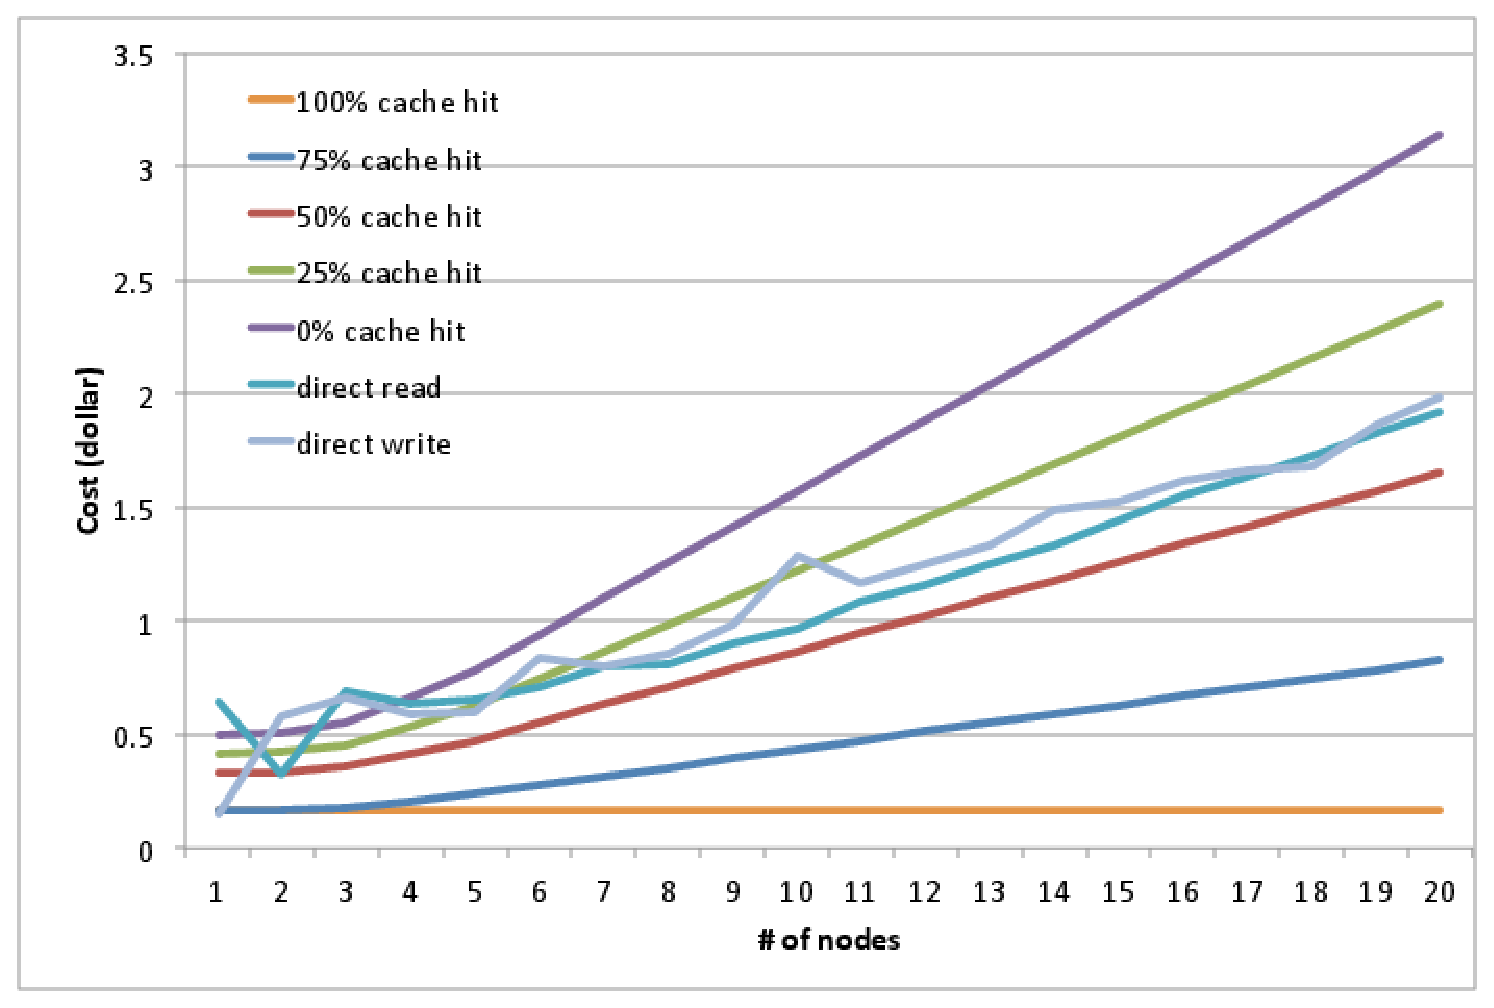
\includegraphics[width=6cm]{../img/cost}
	\caption{cost comparison}
	\label{cost}
\end{figure}

%\begin{figure}[tb]
%	\centering
%	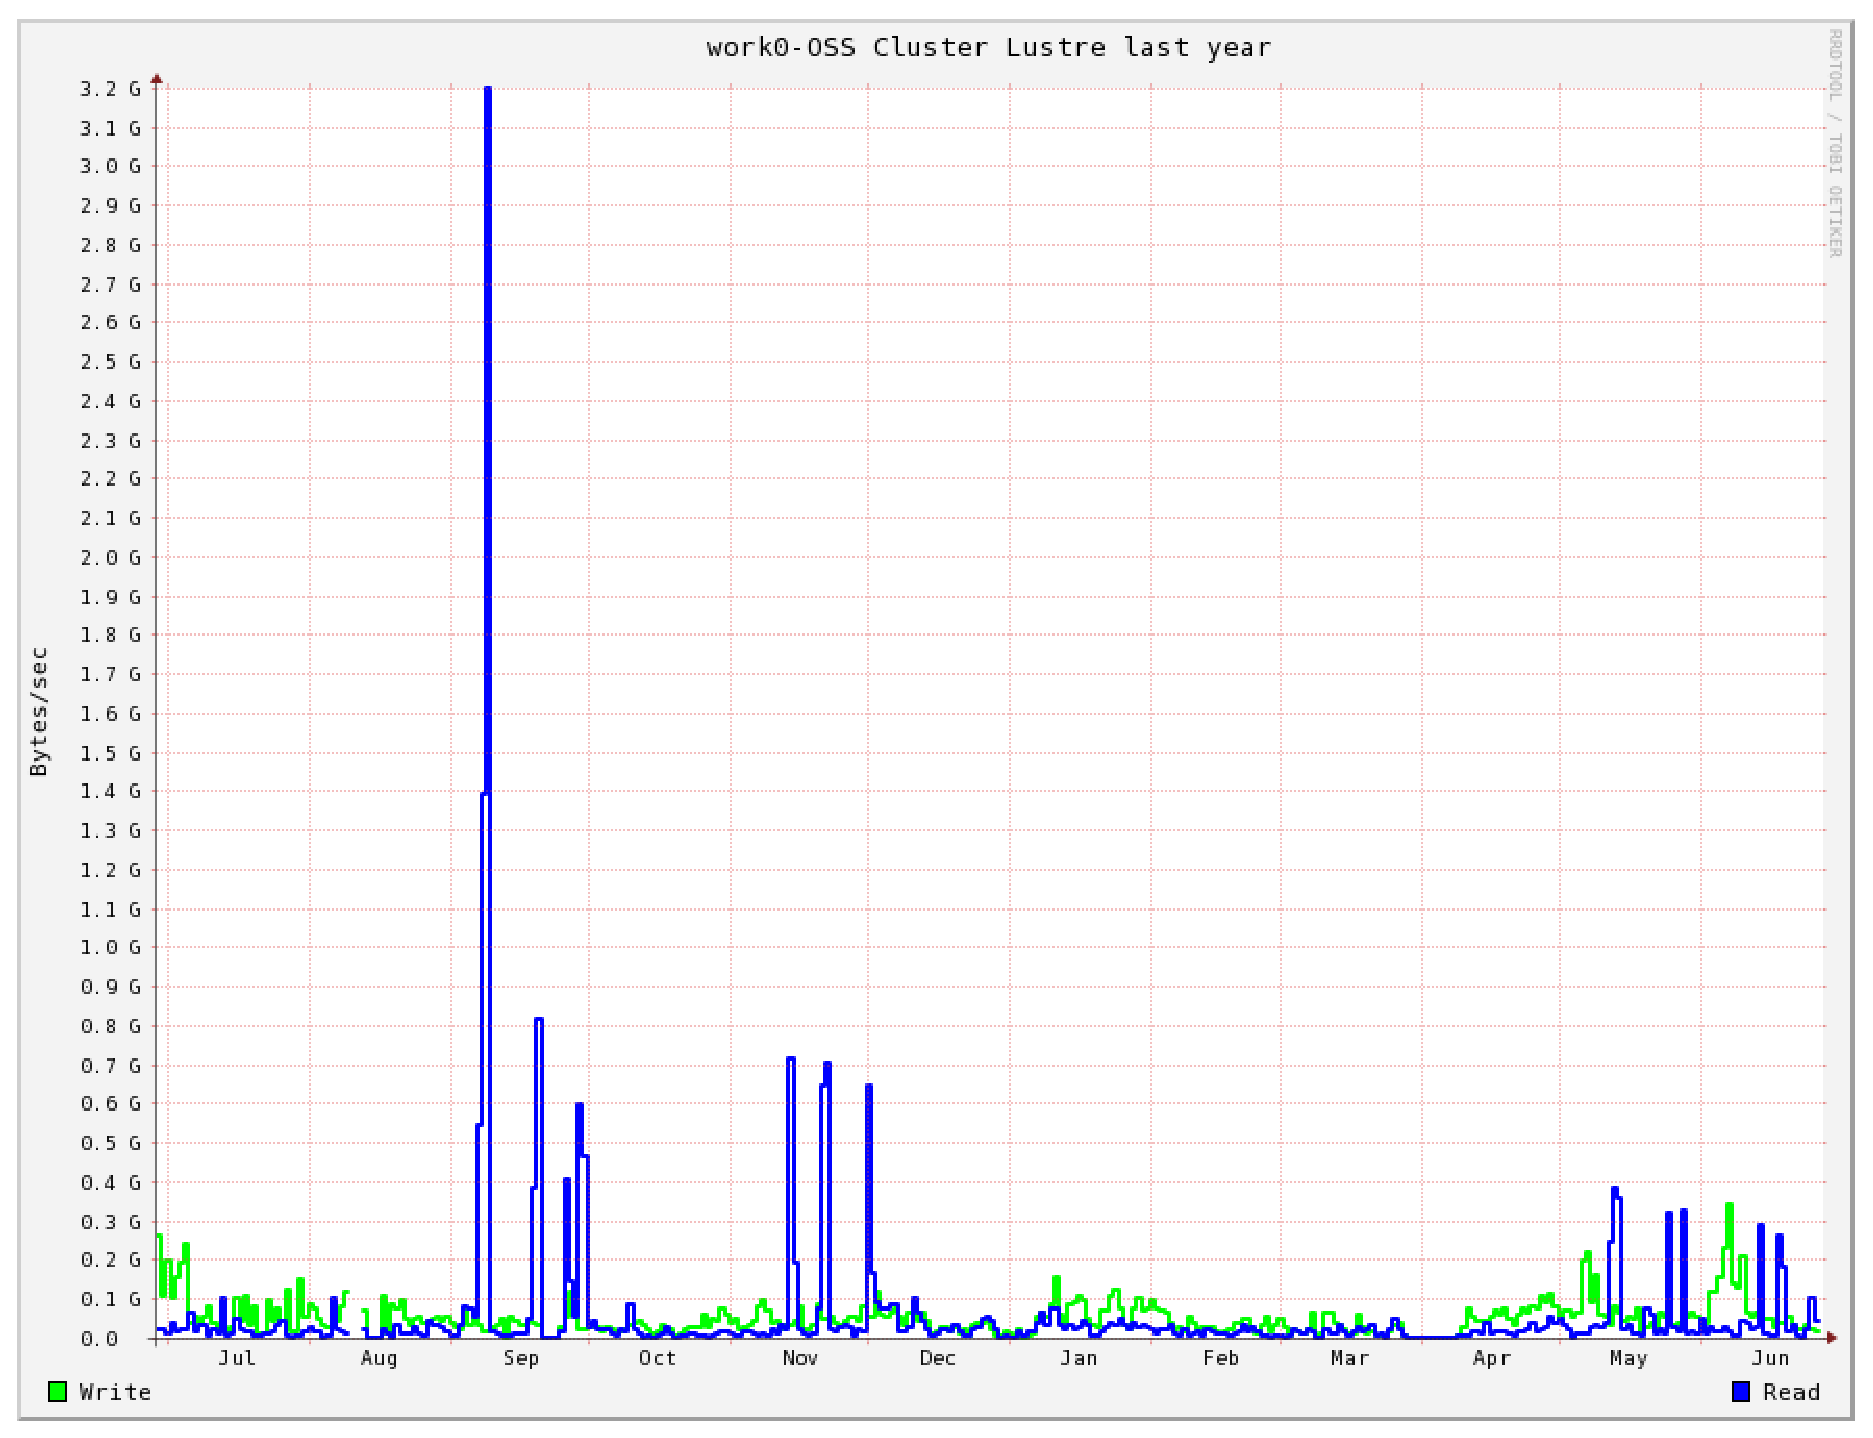
\includegraphics[width=6cm]{tsubamelustre}
%	\caption{TSUBAME Lustre workload}
%	\label{Lustre workload}
%\end{figure}
To evaluate how much federated systems with I/O burst buffers can improve I/O performance and the cost, 
we conduct several simulations based on preliminary performance data taken from several 
benchmarks on both our in-house cluster and Amazon EC2 in a Tokyo region in Section \ref{sec:motivation}.%, using
In the simulations, we assume that computing nodes running on one system read or write files on storage of the other system with the same I/O throughput for both read and write operations.
We also assume an instance type of both the computing nodes and I/O burst buffer nodes is m3.xlarge provided by Amazon EC2.
We compare I/O throughput and overall costs of a system using direct I/O with a system using I/O burst buffer by scaling out up to 20 computing nodes
under different cahch hit rate.
For read operations, the cache hit rate means percentage of data, which is read from buffer queues, to total read size. 
For write operations, the cache hit rate means percentage of data, which is  written to buffer queues before queue becomes full, to total write size.
%Consider we have up to 20 m3.xlarge computing nodes need to transfer data between two systems, 
%Since read and write throughput are the same when using caches on I/O burst buffers, read and write throughput are equal to throughput  between computing nodes and I/O nodes,  we use this throughput value for I/O throughput when use I/O burst buffer..
If read and write are completed via caches on I/O burst buffers
without accessing to remote storage, read and write throughput become 
identical to throughput between a compute node and I/O burst buffer nodes. 
%Thus, we use these throughput for I/O throughput
%m3.medium instance, which has a moderate interconnection network condition and one vcpu with 3.75GiB memory, and
%m3.xlarge instance, which has a high interconnection network condition and 8 vCPUs with 30GiB memory, run Amazon Linux AMI 2014.03.2(HVM) ( Fig.~\ref{throughput TSUBAME}, Fig.~\ref{throughput AMAZON to OURLAB}. Fig.~\ref{point to point connection AMAZON}, Fig.~\ref{point to point connection LAB} ).
%According to these data and definition described above, we use values defined below.

%\begin{center}
%\begin{tabular}[tb]{|c|c|}\hline
%	$D_2$&$E_1$\\\hline
%	8TB/s&1.08Gbit/s(135MB/s)\\\hline
	
%\end{tabular}
%\end{center}
%For throughput between two systems and inside system, from benchmark data, it shows it is hard to achieve a high throughput with only one nodes, and also there is a limit on maximum throughput between two systems and inside system.
%Although incresing nodes can increse throughput before reach the maximum, throughput achieved by each nodes decrease because of conflict.
%For these reason, we use following formular for throughput between two systems and inside system.
%TSUBAME and AMAZON EC2, we use similar model in \cite{ccgrid}:
%\begin{equation}
%throughput=-Ax^2+Bx+C~~ A,B>0\\
%\end{equation}
%we use following equations to determine $A,B,C$
%\begin{equation}
%	\label{throughput equation}
%\begin{cases}
%	-A+B+C=throughput_{one}\\\nonumber
%	\frac{B}{2A}=n_{max}\\\nonumber
%	-An_{max}^2+Bn_{max}+C=throughput_{max}\\
%\end{cases}
%\end{equation}

%Since it is hard for one node to fully utilize Internet and interconnection network bandwidth, according to Fig.~\ref{throughput AMAZON to OURLAB}, we assume that one node can achieve 80\% of maximum bandwidth, and by using I/O burst buffer, can achieve 100\% of maximum bandwidth of both interconnection network and Internet, here interconnection network throughput refers to interconnection network connection throughput in public cloud.

First we compare I/O throughput of direct connection with the throughput of  I/O burst buffer under different cache hit rates assuming that TSUBAME is federated with Amazon EC2.
%In this simulation, we assume that both I/O buffer nodes and computing nodes use m3.xlarge instance and Amazon Linux AMI, and the number of I/O buffer nodes is equal to number of computing nodes in order to achieve a maximum interconnection network throughput.
In this simulation, the number of I/O buffer nodes is equal to the number of computing nodes. This configuration can achieve a maximum I/O throughput.
%In practice, I/O buffer nodes may have a better interconnection network condition than computing nodes, but there also will be many users running their application on large amount of computing nodes, so there can be several computing nodes reading data from or writing data to one I/O nodes, interconnection network bandwidth also can be fully utilized. 
In practice, an I/O buffer node may have higher network throghput than computing nodes, and the throughput can not fully utilized.
But we assume there are many users running their applications on large amount of computing nodes, which concurrently read data from or write data to one I/O bust buffer nodes, the network throughput to I/O buffer is fully utilized.


Fig.~\ref{throughput comparison} and Fig.~\ref{throughput cache rate} shows the throughput comparisons between systems  with and without I/O burst buffers.
For direct I/O, each computing nodes read from and write data to storage directly and concurrently.
When the number of nodes is small, throughput increases as the number of nodes increses.
However, after throughput reach the peak bandwidth between two systems, (120MB/s when number of nodes equals to 10 in our case), 
the throughput becomes flat. %, means Internet bandwidth is fully utilized, and since that I/O is limited by Internet bandwidth.

%For 0\% cache hit cases, since all data should be read from or write back to storage, throughput shows a similar trade, also limited by Internet bandwidth.
In 0\% cache rate cases, since all data should be read from or write back to storage, 
the throughput show a similar trend.%, also limited by Internet bandwidth.
%\kento{Please explain why 0\% is better than others}

The large difference is shown in cache hit 100\%(Fig.~\ref{throughput cache rate}).
In the 100\% cases, all reading files are buffered in buffer queue, 
also buffer queue is not full for writes.
Thus, computing nodes can read from and write to buffer queue each time without accessing to remote storage, 
and the throughput becomens identical to network throughput between computing nodes and I/O buffer nodes.
As we mentioned, network throughput between two instances within Amazon EC2 shows the scalablity even if we increase the pairs of two instances.
I/O throughput can finally achieve around 2700MB/s, which is about 20 times faster than one of direct I/O.% and also 0\%cache hit cases.

However, the 100\% cache rate is an ideal condition, and is not practical in real applications, 
so we also estimate the throughput under 75\%,50\% and 25\% cache rates in Fig.~\ref{throughput cache rate}.
%When there is a cache miss both in read and write, data need to be transfer via both interconnection network and Internet like 0\% cache hit case, and for cache hit, files can be read and written via interconnection network like 100\% cache hit case, so we use two-side Internet throughput($thr_I$) shown in Fig.~\ref{point to point connection LAB}, interconnection network throughput in Amazon($thr_E$) shown in Fig.~\ref{point to point connection AMAZON} and following formular to evaluate throughput for each cache hit rate.
If the cache rate is low, most of reading and writing data need to be transferred via a network between the two systems, i.e, TSUBAME and Amazon EC2.
If applications can use the cache for read or write, I/O throughput can be improved depending on the cache rates.
To estimate the throughput under different cache rates, we use the below model.
 
\[throughput(n)=\frac{1}{MAX\{\frac{{cache\_rate}}{E_2(n)},\frac{1-cache\_rate}{I(n,n)}+\frac{1-cache\_rate}{E_2(n)}\}}\]

we denote $I(n,n)$ as two-side network throughput shown in Fig.~\ref{point to point connection LAB}, 
$E_2(n)$ network throughput within Amazon EC2 shown in Fig.~\ref{point to point connection AMAZON}.

%Result is shown in Fig.~\ref{throughput cache rate}, we can see that althrough, 100\% cache hit achieve a high throughput, even 75\% cache hit is much lower than 100\%, it is because of the great gap between interconnection network bandwidth and Internet bandwidth, also data can transfer faster in interconnection network, user application must wait until cache miss data transferred through Internet.
As shown in Fig.~\ref{throughput cache rate}, we can also see that I/O throughput in 75\% cache rate are much lower than ones of 100\% cache rate.
This is because of a larege gap between network throughput within Amazon EC2 and between the two systems, 
applications must wait until reading or writing data, which is not in caches, are transferred from or to remote storage.

In this simulation we only consider one job use up to 20 computing nodes, but in practice, a large number of computing nodes issue read and write requests concurrently, 
Fig.~\ref{maximum throughput} shows the maximum throughput of different cache rates and direct I/O.
%we can see  that although reading can not achieve a cache hit rate, until buffer queue is full, writing can achieve a extremely high throughput
We can see that write can achieve an extremely high throughput using caches on I/O burst buffer nodes while read can not achieve that high throughput unless target files are in caches.
%If file is buffered in I/O buffer nodes, computing nodes can read it through interconnection network, Fig.~\ref{cache hit}, shows the comparison, we can see that when interconnection network throughput larger than Internet throughput, our solution can achieve a higher I/O throughput, here we assume that interconnection network throuhput can be lower than Internet throughput, but from Fig.~\ref{point to point connection AMAZON}, Fig.~\ref{throughput TSUBAME}, interconnection network usually is faster than Internet, and by using our solution can achieve a high throughput.

%Then, we compare throughput with and without I/O buffer nodes.
%We can see from Fig.~\ref{throughput},although our solution can be limited by both Internet and interconnection network throughput, our I/O burst buffer can fully utilize both Internet and interconnection network. Like previous comparison, when interconnection network is faster than Internet, our solution can achieve a throughput burst even file is not stored in buffer queue in I/O burst buffer like (read data from storage).

%Then we compare overall cost with and without I/O burst buffer, As we mentioned, cost will be determined by both number of nodes and execution time. 
Then we compare overall cost between systems with and without I/O burst buffers.
As we mentioned, the cost is  determined by both the number of nodes and the execution time. 
%As we showed, By using I/O burst buffer, we can achieve a high I/O throughput, and reduce both the execution time and cost, however, I/O buffer node also will be charged, hence we use following formular to evaluate cost
As we showed, by using I/O burst buffers, we can achieve a high I/O throughput, 
and reduce both the execution time and cost.
However, I/O buffer nodes also is charged, hence we use following formular to evaluate the cost.
\[cost(n)=\frac{Data~size}{throughput(n)}\times C_2HM\times n\]
%According to the Amazon pricing policy, m3.xlarge instance is charged  \$0.405 for each hour usage in Asia Pacific(Tokyo).
According to the Amazon pricing policy, m3.xlarge instance is charged by \$0.405 par hour in a Asia Pacific region (Tokyo).
%For direct I/O, nodes is equal to number of computing nodes, but for I/O burst buffer, since we assume that number of I/O nodes is equal to number of computing nodes, here the value of node in above formular will be 2 times number of computing nodes.
For direct I/O, we denotes $n$ as the total number of instances used at Amazon EC2. 
Therefore, $n$ becomes the total number of compute nodes in a system with direct I/O, while $n$ is equal to the total number of both computing nodes and I/O buffer nodes in a system with I/O nodes.
Since we assume that the number of I/O nodes is equal to the number of computing nodes, $n$ for a systen with I/O nodes becomes 2 times higher than $n$ for a system with direct I/O.

Fig.~\ref{cost} shows cost comparison between each cache hit rate and direct I/O, which read or write 100GB data.
As shown in the figure,  we can see that cost grows as the number of nodes grows while there is an exception for 100\% cache hit, which throughput is proportional to nodes number.
As shown in Fig.~\ref{cost}, if cache rate is higher than 50\%, the overall cost using I/O burst buffers become lower than direct I/O, however, if cache rate is lower than 50\%, using I/O burst buffer cost more.

From above simulations, we can see that if we can achieve a high cache rate, we can achieve a high throughput up to 4-20 times faster than direct I/O as well as a low cost up to 2-12 times lower than direct I/O for 20 client nodes.
It is may be difficult for read data cache hit rate to be higher than 50\% (can be possible according to data locality), but it is reasonable for write data can be buffered in buffer queue, since public clouds usually provide instance with large size of memory, and it is easy to achieve a Tera size of buffer queue.
%Since we assume number of I/O buffer node increases as number of computing nodes increases, 
%After that, we compare overall cost when use two-side buffer and one-side buffer, since execution time, in our case, I/O time and I/O throughput will affect cost, for Internet and interconnection network throughput, we use. 
%From Fig.~\ref{cost}, 


\section{Conclusion}
\label{sec:conclusion}

In this paper, we propose a I/O burst buffer architecture to burst I/O throughput, provide throughput-based, cost-based and queue write back model, and provide a simulation based on several benchmarks on TSUBAME supercomputer and AMAZON EC2 public cloud.
we use several nodes in each system as a I/O buffer nodes, and use data buffering to hide the low throughput between two systems connected by Internet.

From simulation result, we showed that our I/O burst buffer can increase I/O throughput when Internet throughput is far smaller than interconnection throughput as well as reducing the overall cost.

For future work, we plan to implement this I/O burst buffer architecture.


\bibliography{../bib/reference}
\end{document}
